%%%% Better Poster latex template example v1.0 (2019/04/04)
%%%% GNU General Public License v3.0
%%%% Rafael Bailo
%%%% https://github.com/rafaelbailo/betterposter-latex-template
%%%% 
%%%% Original design from Mike Morrison
%%%% https://twitter.com/mikemorrison

\documentclass[a0paper,fleqn]{betterposter}

%%%% Uncomment the following commands to customise the format

%% Setting the width of columns
% Left column
%\setlength{\leftbarwidth}{0.25\paperwidth}
% Right column
%\setlength{\rightbarwidth}{0.25\paperwidth}

%% Setting the column margins
% Horizontal margin
%\setlength{\columnmarginvertical}{0.05\paperheight}
% Vertical margin
% \setlength{\columnmarginhorizontal}{0.05\paperheight}
% Horizontal margin for the main column
%\setlength{\maincolumnmarginvertical}{0.15\paperheight}
% Vertical margin for the main column
% \setlength{\maincolumnmarginhorizontal}{0.15\paperheight}

%% Changing font sizes
% Text font
%\renewcommand{\fontsizestandard}{\fontsize{28}{35} \selectfont}
% Main column font
\renewcommand{\fontsizemain}{\fontsize{80}{40} \selectfont}

% Title font
%\renewcommand{\fontsizetitle}{\fontsize{28}{35} \selectfont}
% Author font
%\renewcommand{\fontsizeauthor}{\fontsize{28}{35} \selectfont}
% Section font
%\renewcommand{\fontsizesection}{\fontsize{28}{35} \selectfont}

%% Changing font sizes for a specific text segment
% Place the text inside brackets:
% {\fontsize{28}{35} \selectfont Your text goes here}

%% Changing colors
% Background of side columns
%\renewcommand{\columnbackgroundcolor}{black}
% Font of side columns
%\renewcommand{\columnfontcolor}{gray}
% Background of main column
%\renewcommand{\maincolumnbackgroundcolor}{empirical}
%\renewcommand{\maincolumnbackgroundcolor}{theory}
%\renewcommand{\maincolumnbackgroundcolor}{methods}
%\renewcommand{\maincolumnbackgroundcolor}{intervention}
% Font of main column
%\renewcommand{\maincolumnfontcolor}{gray}
\DeclareFontFamily{U}{skulls}{}
\DeclareFontShape{U}{skulls}{m}{n}{ <-> skull }{}
\newcommand{\skull}{\text{\usefont{U}{skulls}{m}{n}\symbol{'101}}}

\begin{document}	
\betterposter{
%%%%%%%% MAIN COLUMN

\maincolumn{
%%%% Main space

\textbf{Sex:} Males are 250\% more likely to get heart \\ \\ disease. \\ \\ 
\textbf{Age:} 60+ are 66\% more likely to get heart \\ \\ disease. \\ \\
\textbf{Fasting BS:} Above 120 mg/dl are 65\% more \\ \\ likely to get heart disease.\\ \\
\textbf{Resting BP:} Above 145 bpm are 27\% more likely \\ \\ to get heart disease.\\ 
\textbf{Cholesterol:} Above 280 mg/dl are 30\% more \\ \\ likely to get heart disease.\\ \\ 
\textbf{Max Heart Rate:} Below 150 bpm are 132\% more \\ \\ likely to get heart disease.\\ \\ 

\vspace{5cm}
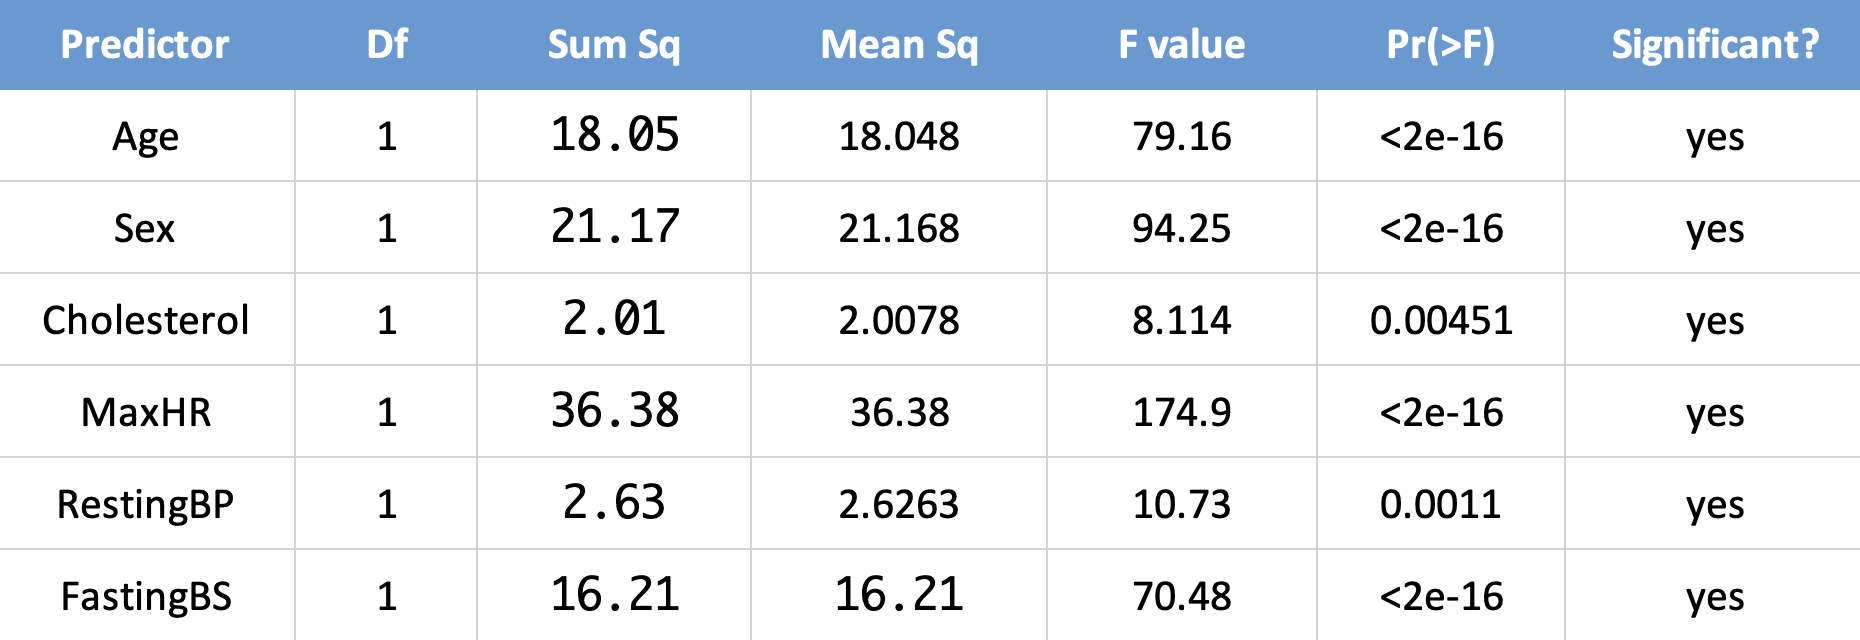
\includegraphics[width=60cm]{anova.png}
\\


}

}{
%%%%%%%% LEFT COLUMN

\title{Heart Failure \\Indications}
\author{Proud Jiao}
\author{Xiaocong Xuan}
\author{Yijie Lu}
\author{Xiaoyan Wei}
\author{Lukas Lam}
\author{Felix Zhou}
\institution{UCLA Statistics}

\section{Relationships \\between Heart Failures \\and Medical Signs }
We investigate variables including: 
\begin{itemize}
\item Age
\item Gender ( M / F )
\item Cholesterol Levels (mm/dl)
\item Fasting Blood Sugar Level (mg/dl)
\item Resting Blood Pressure
\item Max Heart Rate
\end{itemize}

\section{Methods}
We first examined the correlation between variables and heart failures. We then looked at individual distribution grouped by heart failure. In the process of examining the distribution, we fixed missing data and readjusted distributions. On top of that, we ran an analysis of variance to determine which variables contribute the most in affecting the occurrence of heart failure.

\section{Conclusion}
From the anova table, we conclude that age, sex, cholesterol levels, fasting blood sugar level, resting blood pressure, maximum heart rate are all significant indications to determine the occurrence of heart failure.\


%% This fills the space between the content and the logo
%\vfill

%% Institution logo
%
\includegraphics[width=\textwidth]{DeptLogo.png}\\

}{
%%%%%%%% RIGHT COLUMN
\section{Graphs}
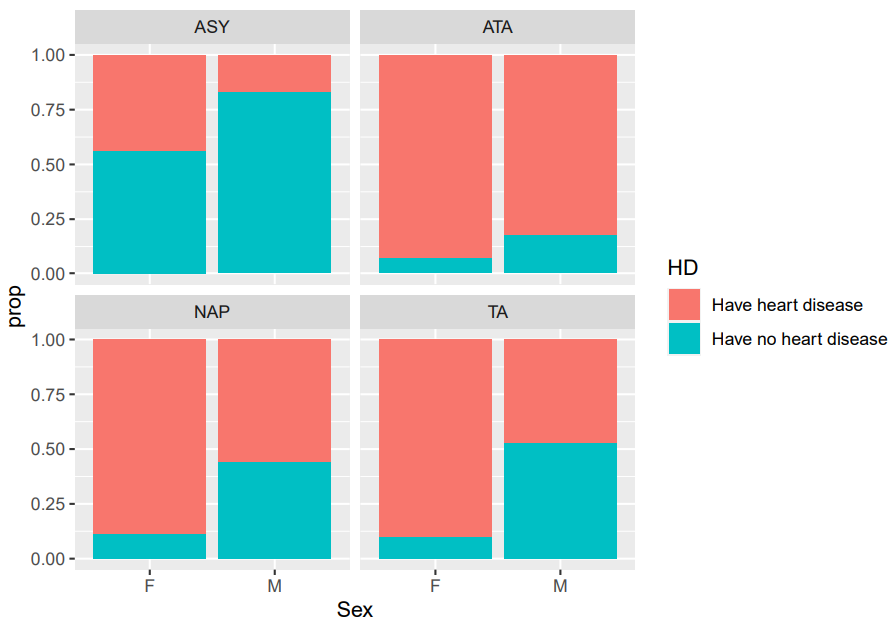
\includegraphics[length=10cm]{directSex.png}
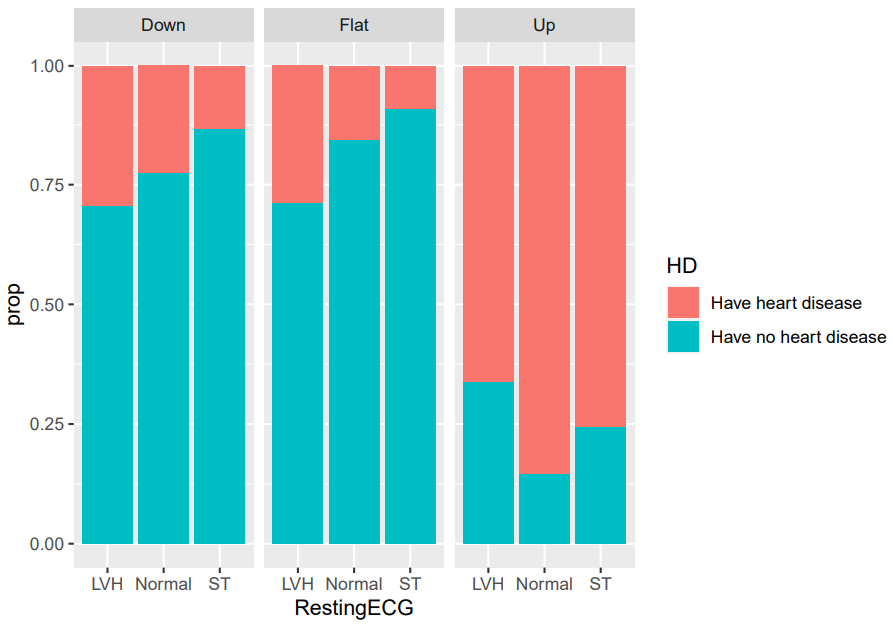
\includegraphics[length=10cm]{directRestingECG.png}
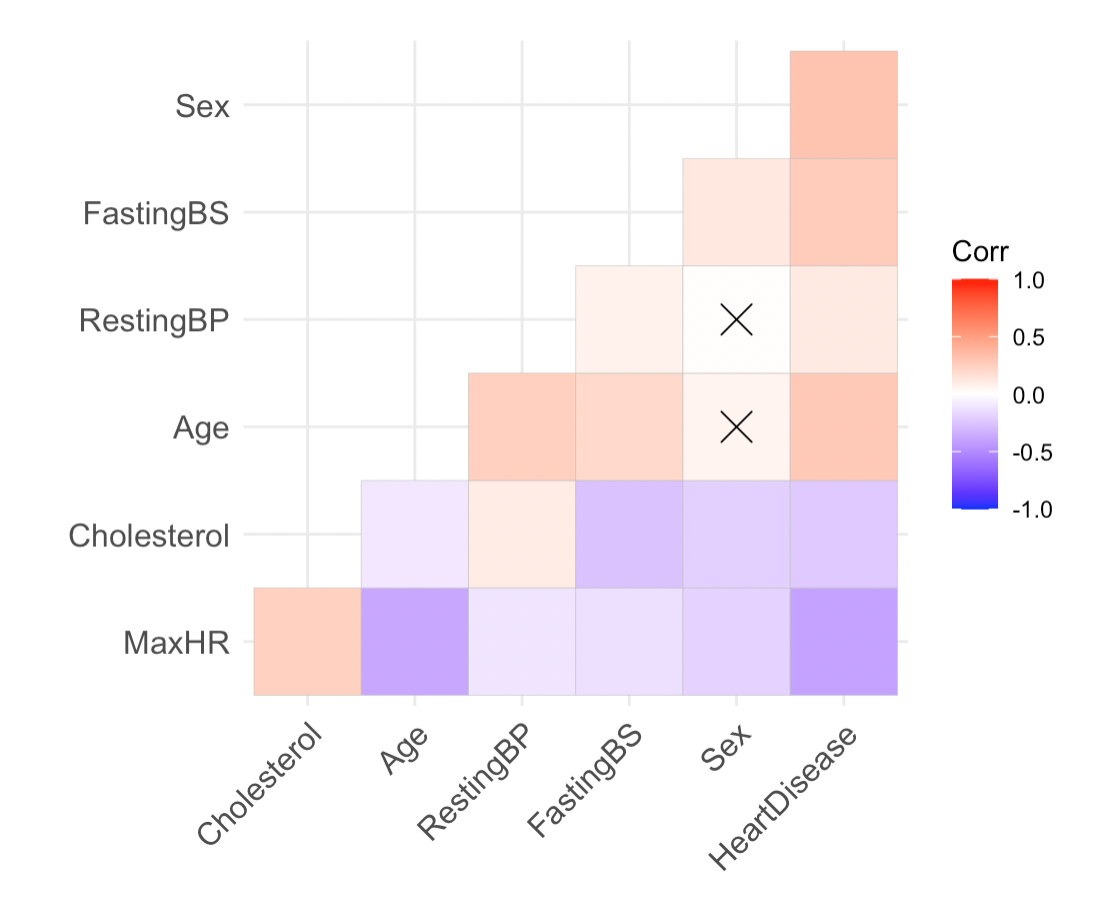
\includegraphics[length=10cm]{cor.png}
\begin{center}

\end{center}

\section{Reference}
Heart Failure Prediction Dataset,\\Kaggle, Fedesoriano, \\https://www.kaggle.com/datasets/\\fedesoriano/heart-failure-prediction
%% This fills the space between the content and the logo
\vfill

%% Institution logo

\includegraphics[width=\textwidth]{UCLA_ds_001.png}\\

}

\end{document}
